\documentclass[xcolor=dvipsnames]{beamer}
\usetheme{Szeged}
\useoutertheme{miniframes}
\useinnertheme{circles}
\definecolor{UBCblue}{rgb}{0.04706, 0.13725, 0.26667} %Allows us to change the beamer's color
\usecolortheme[named=UBCblue]{structure}
%\usefonttheme{structuresmallcapsserif}

\usepackage{amsmath}                                       % Símbolos matemáticos
\usepackage{amsthm}                                        % Símbolos matemáticos
\usepackage{amssymb}
\usepackage{fancyhdr}
\usepackage{lscape}
\usepackage{multirow}
\usepackage{mathtools}
\usepackage{tikz}                                      % Para Tablas. Celdas formadas por múltiples filas
\usepackage{tabularx}
\usepackage{graphics}
\usepackage{color}
\usepackage{float}
\usepackage{lscape}
\usepackage[centerlast]{subfigure}
\usepackage{rotfloat}
\usepackage{hyperref}                                      % Vínculos y personalización del pdf
\usepackage{setspace} 
\usepackage{caption}
\usepackage{graphicx} % Allows to include images
\usepackage{booktabs} % Allows the use of \toprule, \midrule and \bottomrule in tables
%\usepackage{subcaption}
%\usepackage[demo]{graphicx}% delete the demo option in your actual code
%\usepackage{enumitem}
%\usepackage{booktabs}
%\usepackage{xcolor}
% --------------------------------------------------- %
%                    Title + Schedule                 %
% --------------------------------------------------- %
\title[Presentaci\'on]{El efecto traspaso del tipo de cambio hacia los precios de internet}
%\subtitle[]{}
\author[]{Alexandra Marcos \\ Marco Vega \\Erick Lahura}
\institute[PUCP BCRP]{Pontificia Universidad Cat\'olica del Per\'u \\ Banco Central de Reserva del Per\'u}
\date{\today}

% --------------------------------------------------- %
%                  Presentation info	              %
% --------------------------------------------------- %


\begin{document}

\begin{frame}
\titlepage
\end{frame}

\begin{frame}{Esquema de presentaci\'on}
  \tableofcontents
\end{frame}

\section{Preguntas de Investigaci\'on}
\begin{frame}
\textbf{Preguntas de Investigaci\'on: }\\
$\bullet$¿Existe reacci\'on de los precios online como consecuencia de los movimientos del tipo de cambio? \\
$\bullet$¿Depende el nivel de traspaso del tipo de cambio de las caracter\'isticas del propio bien?
\begin{itemize}
	\item Frecuencia de ajuste de precios del bien.
	\item El costo del bien: barato o caro.
	\item La clasificaci\'on del bien.
\end{itemize}
\end{frame}

\section{Motivacion}
\begin{frame}
MOTIVACI\'ON
\end{frame}

\begin{frame}
$\bullet$ El surgimiento del comercio electr\'onico como nuevo segmento del mercado minorista (retail).
\begin{table}[!h]
\begin{tabular}{cc}
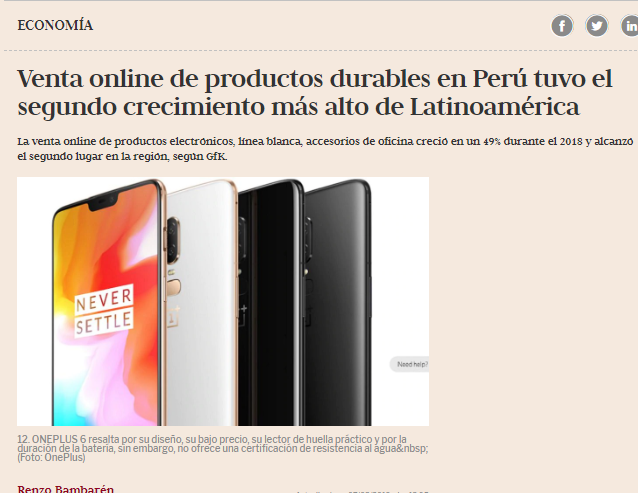
\includegraphics[height=3.99cm, scale = 0.7]{N1.png} &
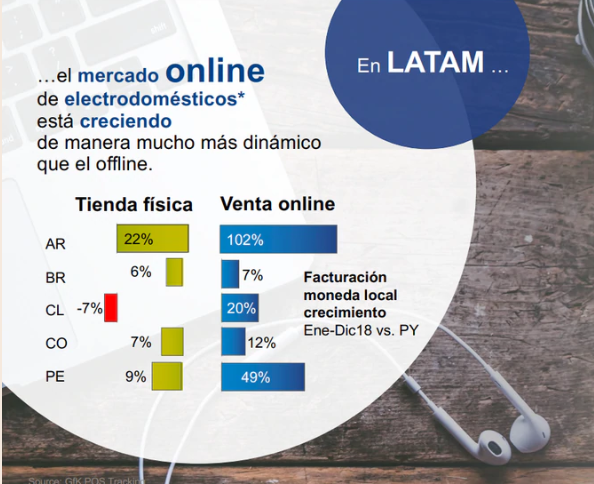
\includegraphics[height=3.99cm, scale =1.0]{N2.png} \\
\end{tabular}
\end{table}
\end{frame}


\begin{frame}
$\bullet$ Un reto hacia el futuro de la pol\'itica monetaria es entender mejor la econom\'ia digital. \\
\begin{enumerate}
	\item E-commerce (Comercio electr\'onico) $\longrightarrow$ \textcolor[rgb]{0.55,0,0}{\textbf{Precios online}}
	\item Fintechs
	\item Dinero digital
\end{enumerate}
\begin{table}[h]
\begin{tabular}{cc}

\includegraphics[height=3.99cm, scale = 0.7]{N3.jpg} &

\includegraphics[height=3.99cm, scale =1.0]{N4.jpg} \\
\end{tabular}
\end{table}
$\bullet$ La escasez de investigaciones que estudien el comportamiento de los precios online. \\
\end{frame}

	
\section{Revision de la Literatura}
\begin{frame}
REVISI\'ON DE LITERATURA
\end{frame}

\begin{frame}

\begin{table}[!h]
\centering
\scalebox{0.5}{
\begin{tabular}{p{3.0cm}m{3em}m{3.0cm}m{3.0cm}m{3.5cm}m{3.0cm}}
  \hline
  % after \\: \hline or \cline{col1-col2} \cline{col3-col4} ...
  \textbf{Autor(es)} & \textbf{Países} & \textbf{Variables relevantes} & \textbf{Controles} & \textbf{Estimación} & \textbf{Datos y muestra} \\
  \hline
  \hline
  Gorodnichenko y Talavera(2017)& Canadá y Estados Unidos & Nivel de los precios relativos Nivel del tipo de cambio nominal & Efectos fijos por producto & Largo plazo: Sin controles: 76.5\% Con controles:67\% & Precios de productos de tiendas minoristas obtenidos de páginas web comparadoras de precios (PWC)Semanal 2008-2013 \\
  \hline
  Cavallo(2018)& Estados Unidos & Variación del indice de precios a nivel de sector. Variación del tipo de cambio nominal& Efectos fijos de individuo y categoria & 26\% bienes sin competencia 44\% Bienes con competencia & P\'agina web de Walmart. 2016-2018. Frecuencia trimestral.\\
  \hline
\end{tabular}
\label{table:1}
}
\end{table}

\end{frame}

\begin{frame}
\begin{table}[!h]
\centering
\scalebox{0.5}{
\begin{tabular}{p{3.5cm}m{3em}m{3.0cm}m{3.0cm}m{3.5cm}m{3.0cm}}
  \hline
  % after \\: \hline or \cline{col1-col2} \cline{col3-col4} ...
  \textbf{Autor(es)} & \textbf{Países} & \textbf{Variables relevantes} & \textbf{Controles} & \textbf{Estimación} & \textbf{Datos y muestra} \\
  \hline
  \hline
  Gorodnichenko y Itshioki(2010)& Canadá y Estados Unidos & Life long passthrough y aggregatte passthrough & Efectos fijos por pa\'is & Largo plazo: El traspaso es casi el doble para productos con mayor frecuencia de cambio & Precios micro del Bureau of Labor Statistics 1994-2005 \\
  \hline
  Gorodnichenko(2018) & Reino Unido y Estados Unidos & Reacci\'on de la frecuencia de ajuste y el tamaño del cambio de los precios.&No reporta & No encuentra reacci\'on de frecuencia de cambio de precios y tamaño del cambio y choque macroecon\'omicos.& PWC. Diaria. Mayo 2010- Febrero 2012. \\
  \hline

\end{tabular}
\label{table:1}
}
\end{table}
\end{frame}

\begin{frame}
\begin{table}[!h]
\centering
\scalebox{0.5}{
\begin{tabular}{p{3.5cm}m{3em}m{3.0cm}m{3.0cm}m{3.5cm}m{3.0cm}}
  \hline
  % after \\: \hline or \cline{col1-col2} \cline{col3-col4} ...
  \textbf{Autor(es)} & \textbf{Países} & \textbf{Variables relevantes} & \textbf{Controles} & \textbf{Estimación} & \textbf{Datos y muestra} \\
  \hline
  \hline
  Castellares(2017)& Perú & Variación del precio del auto(Precio de su ultima aparición contra la primera). Variación del tipo de
cambio nominal & Proxy de calidad: tamaño del precio promedio del auto. Proxy de demanda: búsqueda en Google trends de autos usados. Proxy de competencia: los días que demoro en vender el auto & Sin controles:
27 \% Control de calidad: 35.5 \% Control de competencia: 66.4 \% & Precios de autos usados
publicados en El Comercio Diaria. Semanal 2014-2016.\\
  \hline
 Antoniades y Zaniboni(2016)& Emiratos Árabes Unidos & Variación promedio bimensual de los precios. Variación del tipo de cambio
en la misma frecuencia de los precios. & Proxy de cambios de costo marginal: Cambios en los precios extranjeros. Proxy de cambios en demanda doméstica: Valor de las ventas totales de cada producto & Largo plazo (1 año): 20\% & Precios escaneados de bienes
de rápido consumo de tiendas minoristas. Mensual-Bimensual 2006-2010\\
  \hline

\end{tabular}
\label{table:1}
}
\end{table}
\end{frame}

%\begin{frame}
%Balance de la revision de la literatura: \\
%$\bullet$ Estudios del traspaso a nivel latinoamericano utilizando datos a nivel agregado \\
%$\bullet$ Estudios del traspaso a nivel micro y online mostrar diferencias.
%\end{frame}

\section{Descripci\'on de la base de datos}
\begin{frame}
COMPORTAMIENTO DE LOS PRECIOS ONLINE\\
Descripcion de la base de datos
\end{frame}
\begin{frame}
Base de datos en formato panel
\begin{enumerate}[I]
\item Periodo de estudio
\begin{enumerate}[i]
  \item Inicio: 2016-09-19
  \item Final: 2019-04-30
\end{enumerate}
\item Clasificaci\'on de los productos (Categor\'ias)
%\item [$\bullet$ Bienes "ID" ] 1272
\begin{enumerate}[i]
  \item Audio
  \item Computadores
  \item Electrodom\'estico
  \item Fotograf\'ia
  \item Linea Blanca
  \item Tel\'efonos
  \item Televisores
  \item Electrohogar
\end{enumerate}
\item N\'umero de productos (ID): 1270
\end{enumerate}
\end{frame}

\begin{frame}
\centering
\begin{tabular}{m{2.5cm}m{2cm}m{2cm}m{2cm}}
\toprule
Categor\'ia & N\'umero de productos & N\'umero de observaciones & $\frac{N.Precios}{N.Productos}$ \\
\midrule
Audio & 200 &  87 628 & 438\\
Computadores & 162 &  68 942& 426\\
Electrodom\'esticos & 390 & 174 357 & 447\\
Electrohogar & 17 &   7 427& 437\\
Fotograf\'ia & 69 &  31 144& 451\\
\addlinespace
Linea blanca & 360 & 166 528& 463\\
Tel\'efonos & 39 &  14 857& 381\\
Televisores & 33 &  12 331 & 374\\
\midrule
Total & 1 270 & 563 214 & \\
\bottomrule
\end{tabular}
\end{frame}

\begin{frame}
Histograma del n\'umero de observaciones por ID
\begin{figure}
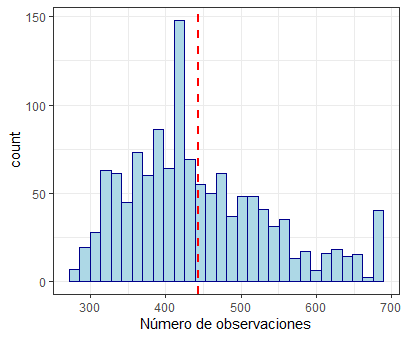
\includegraphics[scale=0.8]{observaciones_producto.png}
\end{figure}
\end{frame}

\begin{frame}
Grafico de densidad del n\'umero de observaciones por categor\'ia
\begin{figure}
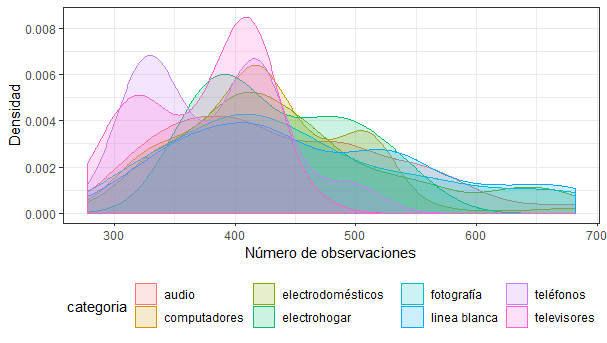
\includegraphics[height=6.00cm, scale=0.69]{observaciones_categoria.png}
\end{figure}
\end{frame}


\begin{frame}
Porcentaje de cambios por ID
\begin{table}[h]
\begin{tabular}{cc}
Precio online & Precio offline\\
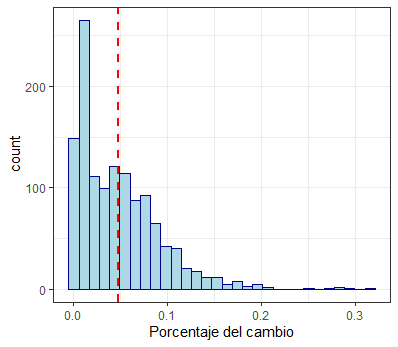
\includegraphics[height=4.59cm]{cambio_producto_internet.png} &
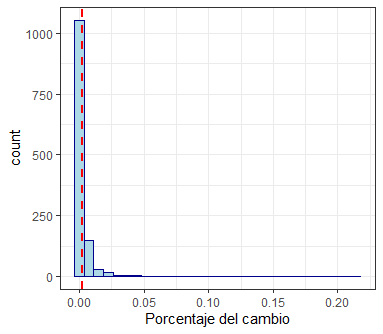
\includegraphics[height=4.59cm]{cambio_producto_normal.png} \\
\end{tabular}
\end{table}
\end{frame}


%\begin{frame}
%Porcentaje de cambios por ID
%\centering
%\begin{tabular}{rrrrrr}
%\toprule
%Min & Q1 & Median & Mean & Q3 & Max\\
%\midrule
%0 & 1.542917 & 5.353921 & 6.722289 & 10.28881 & 42.14286\\
%\bottomrule
%\end{tabular}
%\caption{\label{tab:table-name}Your caption.}
%\end{frame}

\begin{frame}
Frecuencia de cambios por d\'ia: Precio online
\begin{figure}
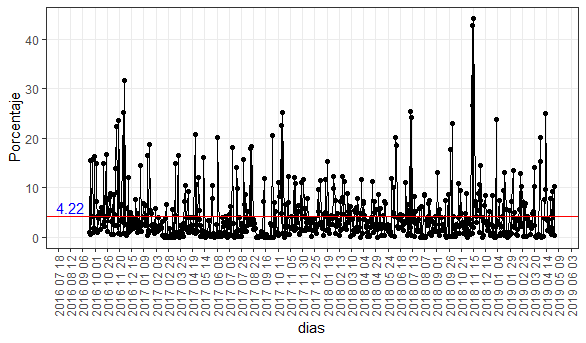
\includegraphics[scale=0.65]{frecuencia_dias_internet.png}
\end{figure}
\end{frame}

\begin{frame}
Frecuencia de cambios por d\'ia: Precio offline
\begin{figure}
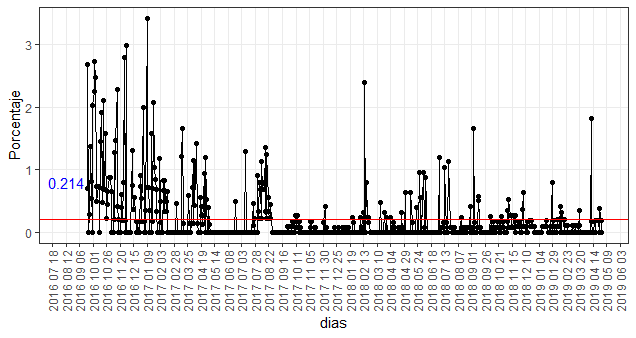
\includegraphics[scale=0.65]{frecuencia_dias_normal.png}
\end{figure}
\end{frame}

%\begin{frame}
%Frecuencia de cambios promedio mensual
%\begin{figure}
%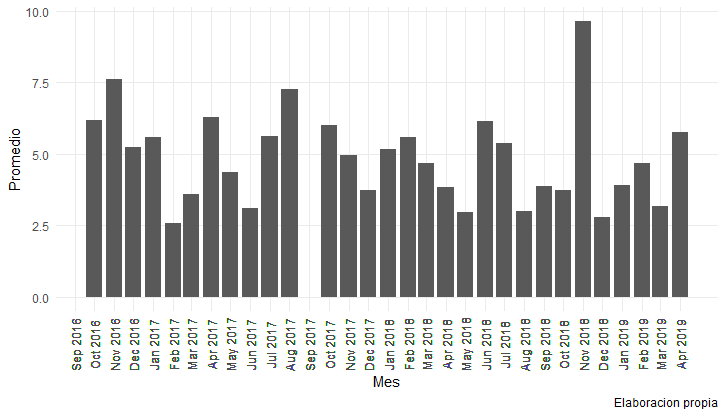
\includegraphics[scale=0.60]{frecuencia_mensual.png}
%\caption{5}
%\end{figure}
%\end{frame}

\begin{frame}
Tamaño del cambio promedio por d\'ia: Precio online
\begin{figure}
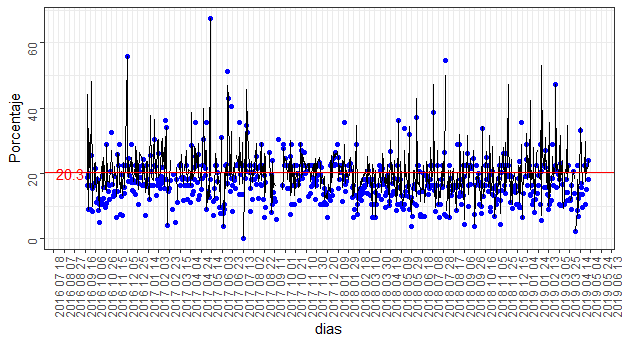
\includegraphics[scale=0.60]{tamano_cambio_promedio_internet.png}
\end{figure}
\end{frame}

\begin{frame}
Tamaño del cambio promedio por d\'ia: Precio offline
\begin{figure}
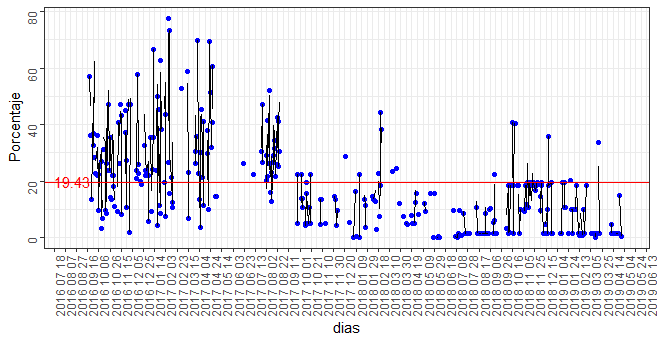
\includegraphics[scale=0.60]{tamano_cambio_promedio_normal.png}
\end{figure}
\end{frame}

\section{Metodologia}
\begin{frame}
Metodolog\'ia
\end{frame}
\begin{frame}
\textbf{Life-Long PassThrough- Modelo General}\\
Este enfoque estima el traspaso del tipo de cambio sobre la vida del bien en la base de datos.\\
\scalebox{0.8}{
\begin{equation}
\Delta P_{it} = \beta_{0} +\beta_{1} \Delta S_{it}  + \beta_{2} \Delta S_{it}*X_{i} + \beta_{3}X_{i} + \beta_{4}Categorias + \beta_{5}Controles + \varepsilon_{it}
\end{equation}}
\begin{itemize}
	\item $\Delta P_{it}$ : Cambio acumulado del precio del bien desde la primera observaci\'on del nuevo precio hasta el siguiente nuevo precio.
	\item $\Delta S_{it}$ : Cambio acumulado del tipo de cambio desde la primera observaci\'on del nuevo precio hasta la ultima observaci\'on del nuevo precio rezagado 20 d\'ias atr\'as.
	\item $X_{i}$ : Frecuencia de ajuste de precios de cada bien, Precio inicial de cada bien.
	\item $Categorias$ : Dummies de la clasificaci\'on de los productos.
	\item $Controles$ : Duracion del precio del bien, Dummy por d\'ias de ofertas.
\end{itemize}
\end{frame}

\begin{frame}
Life-Long PassThrough- Modelo General
\begin{figure}
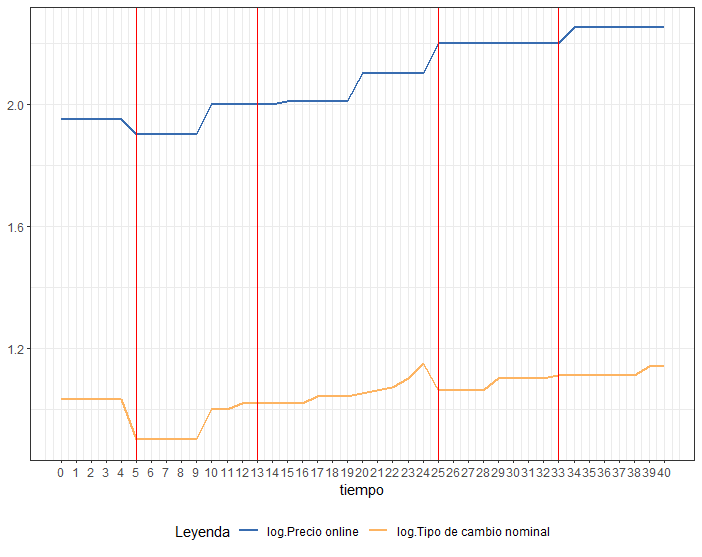
\includegraphics[scale=0.45]{metodologia.png}
\end{figure}
\end{frame}

\begin{frame}
Life-Long PassThrough: Frecuencia del bien
\begin{equation}
\Delta P_{it} = \beta_{1} \Delta S_{it}  + \beta_{2} \Delta S_{it}*f_{i} + \beta_{3}f_{i} + \beta_{4}Categorias + \beta_{5}Controles_{i} + \varepsilon_{it}
\end{equation}
\begin{itemize}
	\item $\Delta P_{it}$ : Cambio acumulado del precio del bien desde la primera observaci\'on del nuevo precio hasta el siguiente nuevo precio.
	\item $\Delta S_{it}$ : Cambio acumulado del tipo de cambio desde la primera observaci\'on del nuevo precio hasta la ultima observaci\'on del nuevo precio rezagado 20 d\'ias atr\'as.
	\item $f_{i}$ : Frecuencia de ajuste de precios de cada bien.
	\item $Categorias$ : Dummies de la clasificaci\'on de los productos.
	\item $Controles$ :  Dummy por d\'ias de ofertas.
\end{itemize}
\end{frame}

\begin{frame}
\begin{table}[!htbp] \centering 
\resizebox{0.8\textwidth}{!}{\begin{tabular}{@{\extracolsep{5pt}} ccccc} 
\\[-1.8ex]\hline 
\hline \\[-1.8ex] 
 & Estimate & Std. Error & t value & Pr(\textgreater \textbar t\textbar ) \\ 
\hline \\[-1.8ex] 
S & $$-$0.366$ & $0.192$ & $$-$1.912$ & $0.056$ \\ 
S*f& $0.082$ & $0.017$ & $4.673$ & $0.00000$ \\ 
f& $0.0002$ & $0.0002$ & $0.746$ & $0.456$ \\ 
DummyOfertas& $$-$0.422$ & $0.004$ & $$-$105.771$ & $0$ \\ 
categoriaAudio & $0.246$ & $0.006$ & $39.680$ & $0$ \\ 
categoriaComputadores & $0.254$ & $0.009$ & $28.256$ & $0$ \\ 
categoriaElectrodomésticos & $0.240$ & $0.004$ & $59.659$ & $0$ \\ 
categoriaElectrohogar & $0.220$ & $0.012$ & $19.030$ & $0$ \\ 
categoriaFotografía & $0.282$ & $0.008$ & $35.693$ & $0$ \\ 
categoriaLinea blanca & $0.244$ & $0.004$ & $62.576$ & $0$ \\ 
categoriaTeléfonos & $0.233$ & $0.007$ & $33.414$ & $0$ \\ 
categoriaTelevisores & $0.240$ & $0.015$ & $16.120$ & $0$ \\ 
\hline \\[-1.8ex] 
\end{tabular}}
\end{table}
\end{frame}

\begin{frame}
Traspaso del tipo de cambio:\\
\begin{equation}
\beta_{1} + \beta_{2}*f_{i}
\end{equation}
Traspaso Medio del tipo de cambio:\\
\begin{equation}
\beta_{1} + \beta_{2}*\overline f
\end{equation}
\begin{equation}
\beta_{1} = -0.37
\end{equation}
\end{frame}

\begin{frame}
\begin{figure}
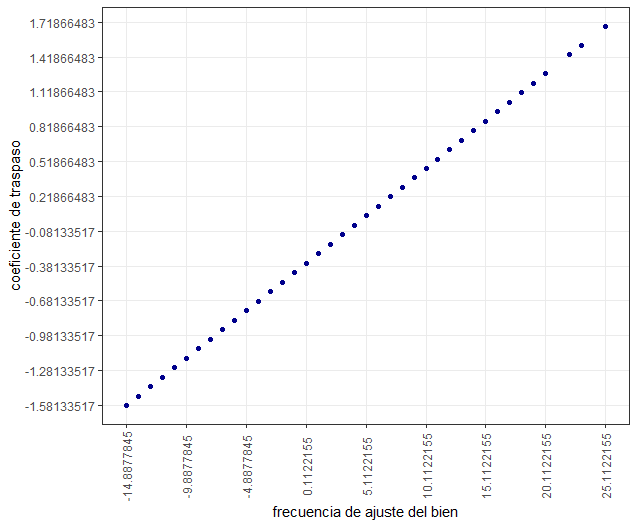
\includegraphics[scale=0.50]{E1.png}
\end{figure}
\end{frame}

\begin{frame}
Life-Long PassThrough: Tamaño del bien
\begin{equation}
\Delta P_{it} = \beta_{1} \Delta S_{it}  + \beta_{2} \Delta S_{it}*P_{i} + \beta_{3}P_{i} + \beta_{4}Categorias + \beta_{5}Controles_{i} + \varepsilon_{it}
\end{equation}
\begin{itemize}
	\item $\Delta P_{it}$ : Cambio acumulado del precio del bien desde la primera observaci\'on del nuevo precio hasta el siguiente nuevo precio.
	\item $\Delta S_{it}$ : Cambio acumulado del tipo de cambio desde la primera observaci\'on del nuevo precio hasta la ultima observaci\'on del nuevo precio rezagado 20 d\'ias atr\'as.
	\item $P_{i}$ : Precio inicial del bien.
	\item $Categorias$ : Dummies de la clasificaci\'on de los productos.
	\item $Controles$ : Duracion del precio del bien, Dummies por d\'ias de ofertas.
\end{itemize}
\end{frame}

\begin{frame} 
\begin{table}[!htbp] \centering 
\resizebox{\textwidth}{!}{\begin{tabular}{@{\extracolsep{5pt}} ccccc} 
\\[-1.8ex]\hline 
\hline \\[-1.8ex] 
 & Estimate & Std. Error & t value & Pr(\textgreater \textbar t\textbar ) \\ 
\hline \\[-1.8ex] 
S & $$-$0.161$ & $0.144$ & $$-$1.115$ & $0.265$ \\ 
S*P & $0.0003$ & $0.00001$ & $29.638$ & $0$ \\ 
P& $$-$0.00002$ & $0.00000$ & $$-$45.789$ & $0$ \\ 
DummyOferta& $$-$0.311$ & $0.004$ & $$-$83.829$ & $0$ \\ 
Duracion & $$-$0.0003$ & $0.00005$ & $$-$5.929$ & $0$ \\ 
categoriAaudio & $0.175$ & $0.005$ & $33.949$ & $0$ \\ 
categoriaComputadores & $0.182$ & $0.008$ & $24.218$ & $0$ \\ 
categoriaElectrodomésticos & $0.171$ & $0.004$ & $48.436$ & $0$ \\ 
categoriaElectrohogar & $0.135$ & $0.009$ & $14.763$ & $0$ \\ 
categoriaFotografía & $0.231$ & $0.007$ & $34.815$ & $0$ \\ 
categoriaLinea blanca & $0.180$ & $0.004$ & $47.033$ & $0$ \\ 
categoriaTeléfonos & $0.129$ & $0.010$ & $13.393$ & $0$ \\ 
categoriaTelevisores & $0.178$ & $0.011$ & $16.118$ & $0$ \\ 
\hline \\[-1.8ex]	
\end{tabular}}
\end{table}
\end{frame}

\begin{frame}
Traspaso del tipo de cambio:\\
\begin{equation}
\beta_{1} + \beta_{2}*P_{i}
\end{equation}
Traspaso Medio del tipo de cambio:\\
\begin{equation}
\beta_{1} + \beta_{2}*\overline P
\end{equation}
\begin{equation}
\beta_{1} + \beta_{2}*982.80 = 0.134
\end{equation}
\end{frame}

\begin{frame}
\begin{figure}
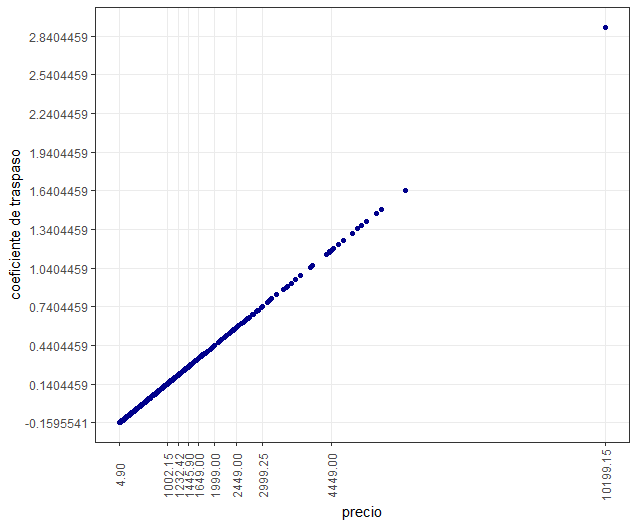
\includegraphics[scale=0.50]{E2.png}
\end{figure}
\end{frame}

\begin{frame}
Life-Long PassThrough: Clasificaci\'on del bien
\begin{equation}
\Delta P_{it} = \beta_{1} \Delta S_{it}  + \beta_{2}Categorias + \beta_{3}\Delta S_{it}*Categorias + \beta_{4}Controles_{i} + \varepsilon_{it}
\end{equation}
\begin{itemize}
	\item $\Delta P_{it}$ : Cambio acumulado del precio del bien desde la primera observaci\'on del nuevo precio hasta el siguiente nuevo precio.
	\item $\Delta S_{it}$ : Cambio acumulado del tipo de cambio desde la primera observaci\'on del nuevo precio hasta la ultima observaci\'on del nuevo precio rezagado 20 d\'ias atr\'as.
	\item $Categorias$ : Dummies de la clasificaci\'on de los productos.
	\item $Controles$ : Duracion del precio del bien, Dummies por d\'ias de ofertas.
\end{itemize}
\end{frame}


\begin{frame}
\begin{table}[!htbp] \centering  
\resizebox{0.80\textwidth}{!}{\begin{tabular}{@{\extracolsep{5pt}} ccccc} 
\\[-1.8ex]\hline 
\hline \\[-1.8ex] 
 & Estimate & Std. Error & t value & Pr(\textgreater \textbar t\textbar ) \\ 
\hline \\[-1.8ex] 
S & $$-$0.394$ & $0.585$ & $$-$0.673$ & $0.501$ \\ 
categoriaAudio & $0.267$ & $0.007$ & $39.115$ & $0$ \\ 
categoriaComputadores & $0.281$ & $0.011$ & $26.514$ & $0$ \\ 
categoriaElectrodomésticos & $0.251$ & $0.005$ & $53.680$ & $0$ \\ 
categoriaElectrohogar & $0.239$ & $0.012$ & $19.918$ & $0$ \\ 
categoriaFotografía & $0.313$ & $0.009$ & $33.376$ & $0$ \\ 
categoriaLinea blanca & $0.259$ & $0.006$ & $46.474$ & $0$ \\ 
categoriaTeléfonos & $0.023$ & $0.010$ & $2.233$ & $0.026$ \\ 
categoriaTelevisores & $0.273$ & $0.016$ & $17.512$ & $0$ \\ 
Duracion & $$-$0.001$ & $0.0001$ & $$-$10.113$ & $0$ \\ 
DummyOferta & $$-$0.421$ & $0.004$ & $$-$96.152$ & $0$ \\ 
P & $$-$0.00001$ & $0.00000$ & $$-$3.374$ & $0.001$ \\ 
f & $0.0005$ & $0.0002$ & $2.285$ & $0.022$ \\ 
S:categoriacomputadores & $$-$0.266$ & $0.848$ & $$-$0.314$ & $0.754$ \\ 
S:categoriaelectrodomésticos & $0.033$ & $0.702$ & $0.046$ & $0.963$ \\ 
S:categoriaelectrohogar & $$-$0.809$ & $1.335$ & $$-$0.606$ & $0.544$ \\ 
S:categoriafotografía & $1.089$ & $0.939$ & $1.160$ & $0.246$ \\ 
S:categorialinea blanca & $0.492$ & $0.710$ & $0.694$ & $0.488$ \\ 
S:categoriateléfonos & $32.836$ & $1.050$ & $31.273$ & $0$ \\ 
S:categoriatelevisores & $1.111$ & $1.993$ & $0.557$ & $0.577$ \\ 
\hline \\[-1.8ex] 
\end{tabular}}
\end{table} 
\end{frame}

\begin{frame}
Traspaso del tipo de cambio por Categoria:\\
\begin{equation}
\beta_{1} + \beta_{3}
\end{equation}
Traspaso del tipo de cambio por categoria:\\
\begin{table}[!htbp] \centering  
\resizebox{0.6\textwidth}{!}{\begin{tabular}{@{\extracolsep{5pt}} lc} 
\\[-1.8ex]\hline 
\hline \\[-1.8ex] 
Categoria & Coeficiente de Traspaso \\ 
\hline \\[-1.8ex] 
Audio & $-0.40$ \\ 
Computadores & $-0.65$\\ 
Electrodomésticos & $-0.36$\\ 
Electrohogar & $-1.20$\\ 
Fotografía & $0.69$ \\ 
Linea blanca & $0.098$ \\ 
Teléfonos & $32.44$ \\ 
Televisores & $0.71$ \\ 
\hline \\[-1.8ex] 
\end{tabular}}
\end{table} 
\end{frame}

\section{Conclusiones}
\begin{frame}
Conclusiones: \\
\begin{itemize}
	\item El traspaso del tipo de cambio aumenta conforme aumenta la frecuencia de ajuste de los precios de cada bien. Frecuencias de ajuste muy bajas puede considerarse traspaso cero.\\
	\item El traspaso del tipo de cambio aumenta conforme aumenta el costo del bien. Mientras más barato sea el bien menor traspaso se encuentra e incluso no existe traspaso. \\
	\item No se encuentra resultados concluyentes con respecto a la relaci\'on del tipo de cambio y la clasificac\'ion del bien como unica explicativa del traspaso.
\end{itemize} 
\end{frame}

\section{Bibliografia}

\end{document} 